\documentclass[serif]{beamer}\usepackage[]{graphicx}\usepackage[]{color}
%% maxwidth is the original width if it is less than linewidth
%% otherwise use linewidth (to make sure the graphics do not exceed the margin)
\makeatletter
\def\maxwidth{ %
  \ifdim\Gin@nat@width>\linewidth
    \linewidth
  \else
    \Gin@nat@width
  \fi
}
\makeatother

\definecolor{fgcolor}{rgb}{0.345, 0.345, 0.345}
\newcommand{\hlnum}[1]{\textcolor[rgb]{0.686,0.059,0.569}{#1}}%
\newcommand{\hlstr}[1]{\textcolor[rgb]{0.192,0.494,0.8}{#1}}%
\newcommand{\hlcom}[1]{\textcolor[rgb]{0.678,0.584,0.686}{\textit{#1}}}%
\newcommand{\hlopt}[1]{\textcolor[rgb]{0,0,0}{#1}}%
\newcommand{\hlstd}[1]{\textcolor[rgb]{0.345,0.345,0.345}{#1}}%
\newcommand{\hlkwa}[1]{\textcolor[rgb]{0.161,0.373,0.58}{\textbf{#1}}}%
\newcommand{\hlkwb}[1]{\textcolor[rgb]{0.69,0.353,0.396}{#1}}%
\newcommand{\hlkwc}[1]{\textcolor[rgb]{0.333,0.667,0.333}{#1}}%
\newcommand{\hlkwd}[1]{\textcolor[rgb]{0.737,0.353,0.396}{\textbf{#1}}}%

\usepackage{framed}
\makeatletter
\newenvironment{kframe}{%
 \def\at@end@of@kframe{}%
 \ifinner\ifhmode%
  \def\at@end@of@kframe{\end{minipage}}%
  \begin{minipage}{\columnwidth}%
 \fi\fi%
 \def\FrameCommand##1{\hskip\@totalleftmargin \hskip-\fboxsep
 \colorbox{shadecolor}{##1}\hskip-\fboxsep
     % There is no \\@totalrightmargin, so:
     \hskip-\linewidth \hskip-\@totalleftmargin \hskip\columnwidth}%
 \MakeFramed {\advance\hsize-\width
   \@totalleftmargin\z@ \linewidth\hsize
   \@setminipage}}%
 {\par\unskip\endMakeFramed%
 \at@end@of@kframe}
\makeatother

\definecolor{shadecolor}{rgb}{.97, .97, .97}
\definecolor{messagecolor}{rgb}{0, 0, 0}
\definecolor{warningcolor}{rgb}{1, 0, 1}
\definecolor{errorcolor}{rgb}{1, 0, 0}
\newenvironment{knitrout}{}{} % an empty environment to be redefined in TeX

\usepackage{alltt}
\usetheme{EPA}
\usepackage{graphicx}
\usepackage{xcolor}
\usepackage{tikz}
\usetikzlibrary{shadows,arrows,positioning}

\newcommand{\emtxt}[1]{\textbf{\textit{#1}}}

\tikzstyle{block} = [rectangle, draw, text width=7em, text centered, rounded corners, minimum height=3em, minimum width=7em, top color = white, bottom color=brown!30,  drop shadow]

% knitr setup


\IfFileExists{upquote.sty}{\usepackage{upquote}}{}
\begin{document}

\title[Shiny Overview]{\textbf{An overview of Shiny applications using R and RStudio}\vspace{-0.15in}}
\author[M. Beck]{Marcus W. Beck\inst{1}}

\institute[USEPA]{\inst{1} USEPA National Health and Environmental Effects Research Laboratory, Gulf Ecology Division, \href{mailto:beck.marcus@epa.gov}{beck.marcus@epa.gov}}

\date{Dec. 10, 2015}

%%%%%%
\begin{frame}
\titlepage
\end{frame}

%%%%%%
\begin{frame}{Who am I?}
\begin{itemize}
\item ORISE post-doc for 2.5 years, fed postdoc since last week \\~\\
\item NHEERL Gulf Ecology Division \\~\\
\item Research focus on water quality assessment and indicator development \\~\\
\item Specific interests in statistical modelling, data assimilation, graphics  \\~\\
\end{itemize}
\end{frame}

%%%%%%
\begin{frame}{Who am I?}
\begin{itemize}
\item R user since 2007 \\~\\
\item Maintainer of two packages on CRAN: \\~\\
\end{itemize}
\begin{columns}[T]
\begin{column}{0.45\textwidth}
\emtxt{SWMPr}\\~\\
Tools for retrieving, organizing, and analyzing data from the System Wide Monitoring Program of the National Estuarine Research Reserve System. 
\end{column}
\begin{column}{0.45\textwidth}
\emtxt{NeuralNetTools} \\~\\
Visualization and analysis tools to aid in the interpretation of neural network models
\end{column}
\end{columns}
\end{frame}

%%%%%%
\begin{frame}{Reproducible research workflow}
General workflow for \emtxt{reproducible research} - reproduce results from an experiment or analysis conducted by another.\\~\\
From Wikipedia... `The ultimate product is the \emtxt{paper along with the full computational environment} used to produce the results in the paper such as the code, data, etc. that can be \emtxt{used to reproduce the results and create new work} based on the research.'\\~\\
\begin{columns}
\begin{column}{0.25\textwidth}
\centerline{
\includegraphics[width = \textwidth]{fig/Rlogo.png}}
\end{column}
\begin{column}{0.25\textwidth}
\centerline{
\includegraphics[width = \textwidth]{fig/RStudio.png}}
\end{column}
\begin{column}{0.25\textwidth}
\centerline{
\includegraphics[width = \textwidth]{fig/knit-logo.png}}
\end{column}
\begin{column}{0.25\textwidth}
\centerline{
\includegraphics[width = \textwidth]{fig/octocat.png}}
\end{column}
\end{columns}
\end{frame}

%%%%%%
\begin{frame}{Reproducible research workflow}
\begin{columns}
\begin{column}{0.23\textwidth}
\centerline{
\includegraphics[width = \textwidth]{fig/Rlogo.png}}
\end{column}
\begin{column}{0.23\textwidth}
\centerline{
\includegraphics[width = \textwidth]{fig/RStudio.png}}
\end{column}
\begin{column}{0.23\textwidth}
\centerline{
\includegraphics[width = \textwidth]{fig/knit-logo.png}}
\end{column}
\begin{column}{0.23\textwidth}
\centerline{
\includegraphics[width = \textwidth]{fig/octocat.png}}
\end{column}
\end{columns}
\vspace{0.2in}
The use of these tools increases transparency and transfer of information \emtxt{= better science}\\~\\
Data prep, analysis, report, and sharing can all be done in RStudio IDE
\end{frame}

%%%%%%
\begin{frame}{Introduction to Shiny}
Where does Shiny fit with reproducible research? \\~\\
Shiny is a web application framework for R \\~\\
\begin{columns}
\begin{column}{0.7\textwidth}
\begin{itemize}
\item From the command line to a graphical user interface 
\item Make your code interactive 
\item Do not need to know anything about web programming
\item Integrated very well with R studio \\~\\
\end{itemize}
\end{column}
\begin{column}{0.2\textwidth}
\centerline{
\includegraphics[width = \textwidth]{fig/shiny_logo.png}}
\end{column}
\end{columns}
\vspace{0.16in}
Tools like Shiny improve \emtxt{accessibility} and \emtxt{communication} 
\end{frame}

%%%%%%
\begin{frame}{Introduction to Shiny}
A minimal working example...\\~\\
\begin{center}
\includegraphics<1>[width = 0.7\textwidth]{fig/mwe1.png}
\includegraphics<2>[width = 0.7\textwidth]{fig/mwe2.png}
\includegraphics<3>[width = 0.7\textwidth]{fig/mwe3.png}
\includegraphics<4>[width = 0.7\textwidth]{fig/mwe4.png}
\end{center}
\end{frame}

%%%%%%
\begin{frame}[t]{Introduction to Shiny}
What's under the hood? Two files... \emtxt{server.R}\\~\\
\centerline{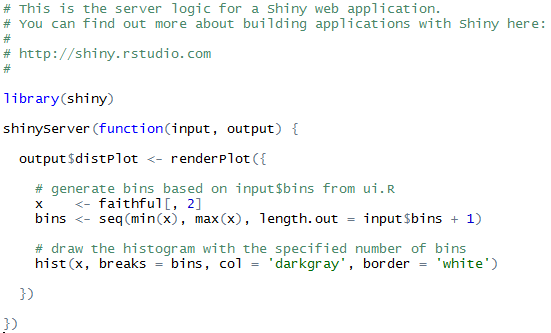
\includegraphics[width = 0.65\textwidth]{fig/serverex.png}}
\end{frame}

%%%%%%
\begin{frame}[t]{Introduction to Shiny}
What's under the hood? Two files... \emtxt{ui.R}\\~\\
\centerline{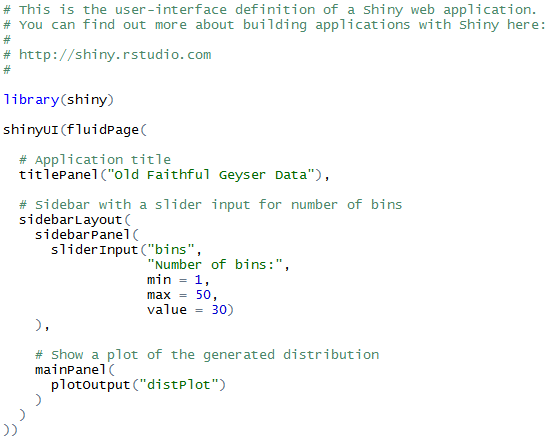
\includegraphics[width = 0.65\textwidth]{fig/uiex.png}}
\end{frame}

%%%%%%
\begin{frame}[t]{Introduction to Shiny}
The files contain only R code! \\~\\
\begin{itemize}
\item \emtxt{server.R}: Contains instructions to build the content, e.g., plots, functions, etc.\\~\\
\item \emtxt{ui.R}: Controls the layout and appearance of the app, i.e., panel types, widgets, etc. \\~\\
\end{itemize}
Executing a Shiny app will run both scripts, user input to \emtxt{ui.R} sent to \emtxt{server.R}, output from \emtxt{server.R} sent to \emtxt{ui.R} for display
\end{frame}

%%%%%%
\begin{frame}[t, fragile]{Introduction to Shiny}
Step 1: User input to \emtxt{ui.R}, `bins'
\small
\begin{kframe}
\begin{alltt}
\hlkwd{sliderInput}\hlstd{(}\hlstr{"bins"}\hlstd{,}
            \hlstr{"Number of bins:"}\hlstd{,}
            \hlkwc{min} \hlstd{=} \hlnum{1}\hlstd{,}
            \hlkwc{max} \hlstd{=} \hlnum{50}\hlstd{,}
            \hlkwc{value} \hlstd{=} \hlnum{30}\hlstd{)}
\end{alltt}
\end{kframe}
\begin{center}
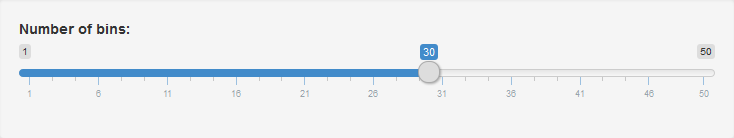
\includegraphics[width = \textwidth]{fig/sliderinput.png}
\end{center}
\end{frame}

%%%%%%
\begin{frame}[t, fragile]{Introduction to Shiny}
Step 2: Input from \emtxt{ui.R} sent to \emtxt{server.R}, executed
\small
\begin{kframe}
\begin{alltt}
\hlcom{# generate bins based on input from ui.R}
\hlstd{x} \hlkwb{<-} \hlstd{faithful[,} \hlnum{2}\hlstd{]}
\hlstd{bins} \hlkwb{<-} \hlkwd{seq}\hlstd{(}\hlkwd{min}\hlstd{(x),} \hlkwd{max}\hlstd{(x),} \hlkwc{length.out} \hlstd{= input}\hlopt{$}\hlstd{bins} \hlopt{+} \hlnum{1}\hlstd{)}

\hlcom{# draw the histogram with the specified number of bins}
\hlkwd{hist}\hlstd{(x,} \hlkwc{breaks} \hlstd{= bins,} \hlkwc{col} \hlstd{=} \hlstr{'darkgray'}\hlstd{,} \hlkwc{border} \hlstd{=} \hlstr{'white'}\hlstd{)}
\end{alltt}
\end{kframe}
\normalsize
Step 3: Output from \emtxt{server.R} sent to \emtxt{ui.R}, plotted on app
\small
\begin{kframe}
\begin{alltt}
\hlkwd{plotOutput}\hlstd{(}\hlstr{"distPlot"}\hlstd{)}
\end{alltt}
\end{kframe}
\normalsize
Step 4: Rinse and repeat
\end{frame}

%%%%%%
\begin{frame}{Introduction to Shiny}
This style of programming and execution is \emtxt{reactive} - re-executes automaticallly when inputs change \\~\\
This has tremendous value: \\~\\
\begin{itemize}
\item Quick code execution after initial setup \\~\\
\item Ease of use for others given application infrastructure \\~\\
\item Ease of use for the developer - no knowledge of web programming needed
\end{itemize}
\end{frame}

%%%%%%
\begin{frame}[t]{Introduction to Shiny}
Shiny applications are very flexible: \href{http://shiny.rstudio.com/gallery/widget-gallery.html}{widgets}
\begin{center}
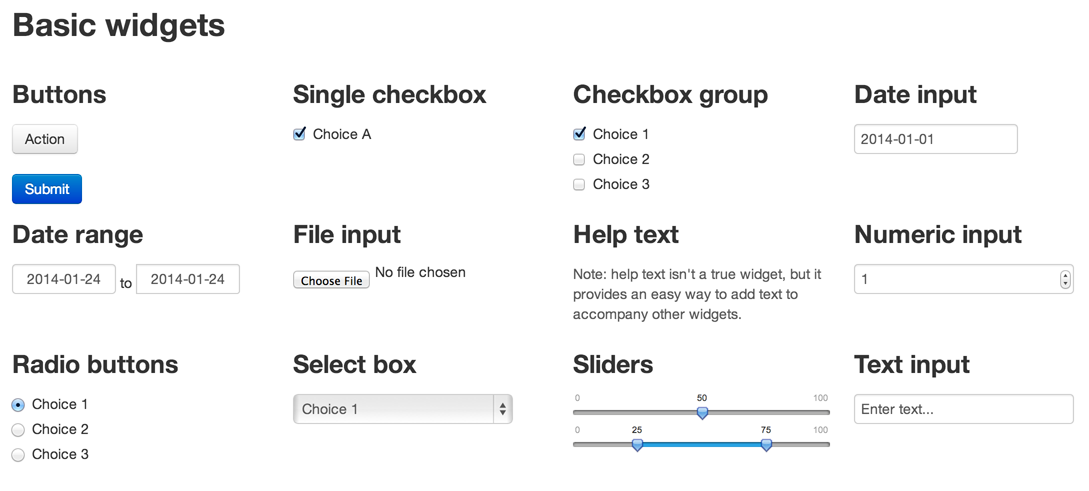
\includegraphics[width = \textwidth]{fig/widgets.png}
\end{center}
\end{frame}

%%%%%%
\begin{frame}[t]{Introduction to Shiny}
Shiny applications are very flexible: outputs
\begin{center}
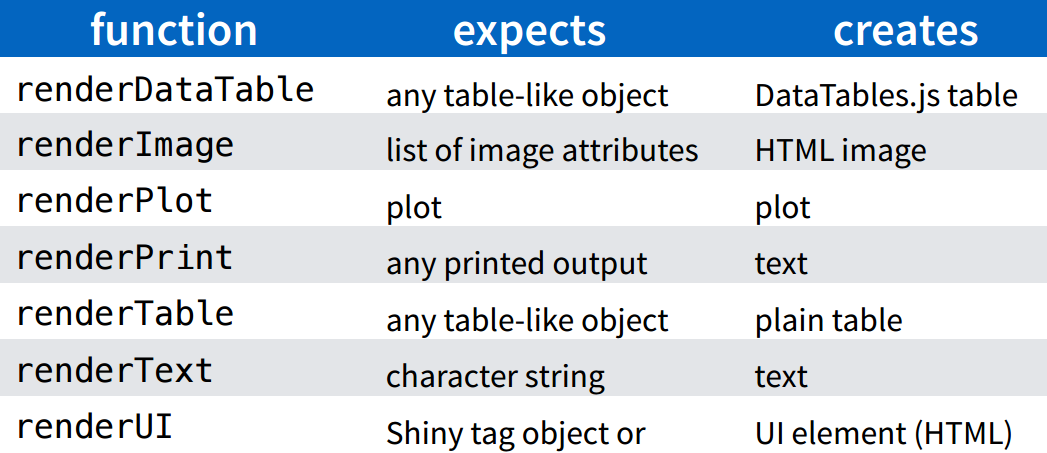
\includegraphics[width = \textwidth]{fig/outputs.png}
\end{center}
\end{frame}

%%%%%
\begin{frame}[t]{Introduction to Shiny}
Shiny applications are very flexible: use of HTML or Javascipt libraries \\~\\
\begin{itemize}
\item Refined layouts: \href{https://rstudio.github.io/shinydashboard/}{shinydashboard}, \href{http://www.htmlwidgets.org/}{htmlwidgets}, \href{https://ebailey78.github.io/shinyBS/}{shinyBS} \\~\\
\item Interacive graphics: \href{https://rstudio.github.io/dygraphs/}{dygraphs}, \href{http://hrbrmstr.github.io/metricsgraphics/}{metricsgraphics}, \href{https://plot.ly/r/shiny-tutorial/}{plotly} \\~\\
\item Mapping: \href{https://rstudio.github.io/leaflet/}{leaflet} \\~\\
\end{itemize}
Use of these libraries can create applications comparable to any other web application for data viz
\end{frame}

%%%%%%
\begin{frame}{Introduction to Shiny}
Apps are easily shared.... \\~\\
For the \emtxt{single} user: \\~\\
\begin{itemize}
\item Local RStudio `project' as a standalone working directory \\~\\
\end{itemize}
For \emtxt{multiple} users: \\~\\
\begin{itemize}
\item As a web application on your server, requires Shiny Server \\~\\
\item As a web application hosted on \url{http://www.shinyapps.io/}
\end{itemize}
\end{frame}

%%%%%%
\begin{frame}{Shiny Examples}
Research application: Evaluating a statistical model to isolate and remove variance components from a time series\\~\\
\emtxt{Scenario}: Time series of dissolved oxygen provide information on ecosystem processes in aquatic systems \\~\\
\emtxt{Problem}: These time series are assumed to measure biological production/respiration, but noise from tidal cycles in coastal systems 
\end{frame}

%%%%%%
\begin{frame}{Shiny Examples}
A tidal and dissolved oxygen time series at Sapelo Island, Georgia
\centerline{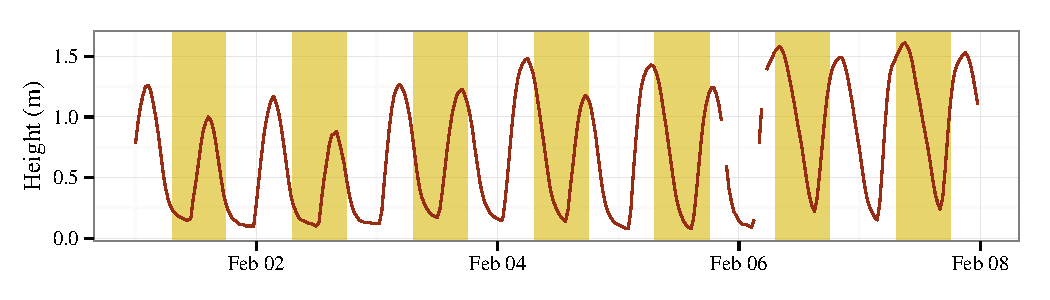
\includegraphics[width = 0.9\textwidth]{fig/saptide.pdf}}
\centerline{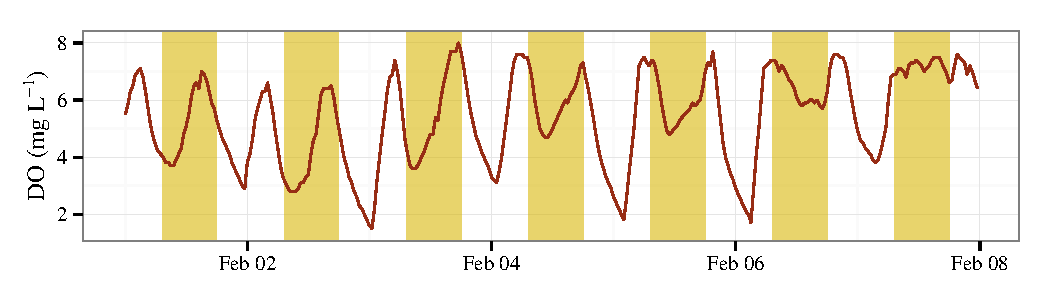
\includegraphics[width = 0.9\textwidth]{fig/sapdo.pdf}}
\end{frame}

%%%%%%
\begin{frame}{Shiny Examples}
Grid-based evaluation of the statistical model using simulated time series and varying model paremeters \\~\\
\begin{itemize}
\item Time series varying by 4 characteristics, 3 levels per characteristic \\~\\
\item Model parameters varying by 3 characeristics, 3 levels per characterisic \\~\\
\end{itemize}
2187 unique combinations: Very challenging to evaluate results, use Shiny!
\end{frame}

%%%%%%
\begin{frame}{Shiny Examples}
\centerline{\url{https://beckmw.shinyapps.io/detiding_sims/}}
\vspace{0.1in}
\centerline{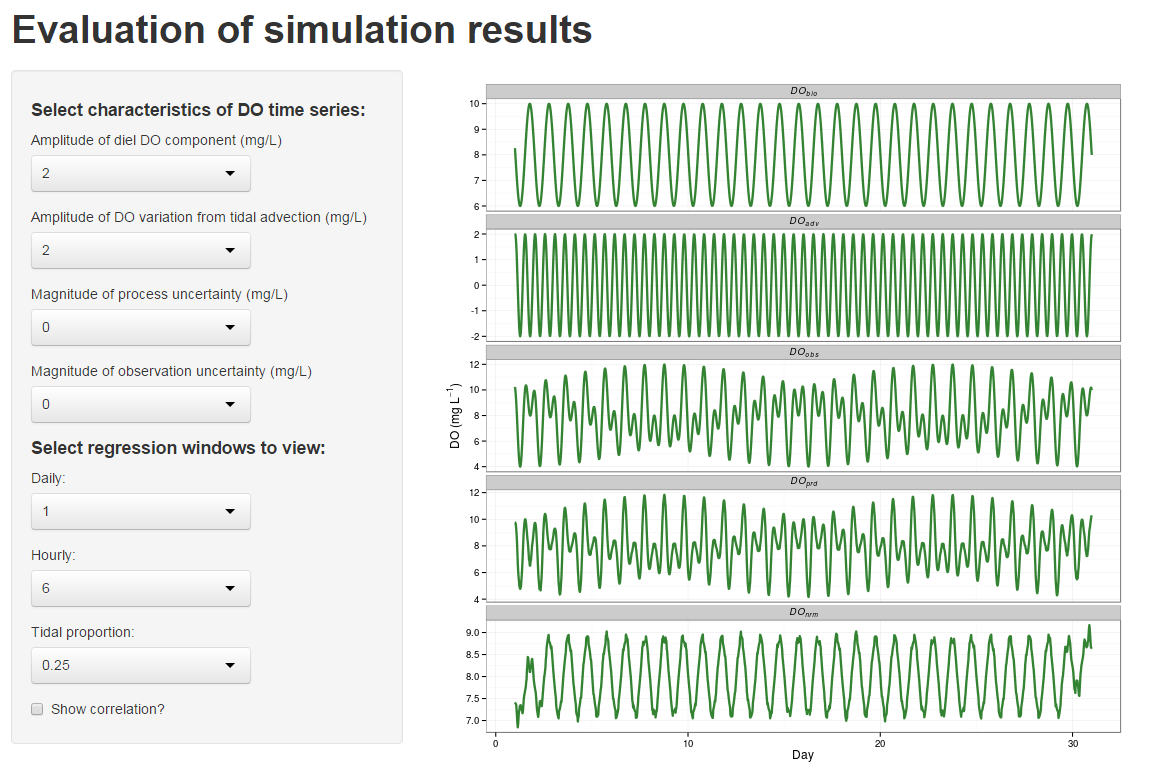
\includegraphics[width = 0.8\textwidth]{fig/shinyex1.png}}
\end{frame}

%%%%%%
\begin{frame}{Shiny Examples}
Management application: Spatial and temporal assessment of water quality trends in NOAA estuary reserves\\~\\
{\bf NERRS}\\
National Estuarine Research Reserve System, established by Coastal Zone Management Act of 1972. Focus on \emtxt{long-term research}, \emtxt{monitoring}, \emtxt{education}, and \emtxt{stewardship} for more effective coastal management.\\~\\
{\bf SWMP}\\
System Wide Monitoring Program, initiated in 1995 to provide \emtxt{continuous monitoring} data at over 140 stations in each of the 28 NERRS reserves \\~\\
\end{frame}

%%%%%%
\begin{frame}{Shiny Examples}
Location of NERRS estuary reserves with SWMP data\\~\\
\centerline{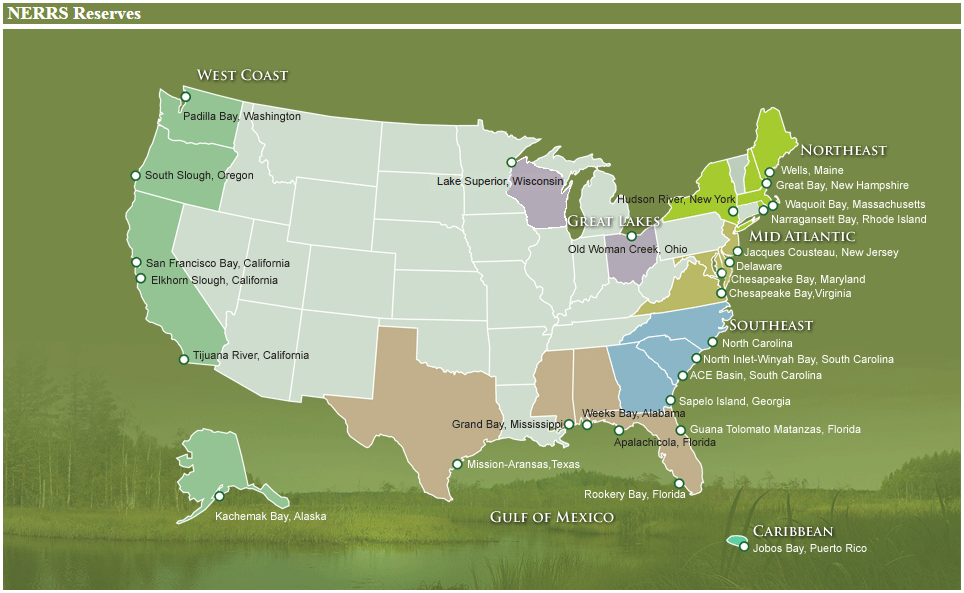
\includegraphics[width = 0.9\textwidth]{fig/NERRS_locations.png}}
\end{frame}

%%%%%%
\begin{frame}{Shiny Examples}
Although SWMP data have been collected and processed using standardized methods... \\~\\
\begin{itemize}
\item Long-term trends have not been evaluated between-reserves in several years \\~\\
\item Tools for simple trend analysis and visualization have been lacking \\~\\
\end{itemize}
\emtxt{Solution}: Use Shiny to bring results to users!
\end{frame}

%%%%%%
\begin{frame}{Shiny Examples}
\centerline{\url{https://beckmw.shinyapps.io/swmp_comp/}}
\vspace{0.1in}
\centerline{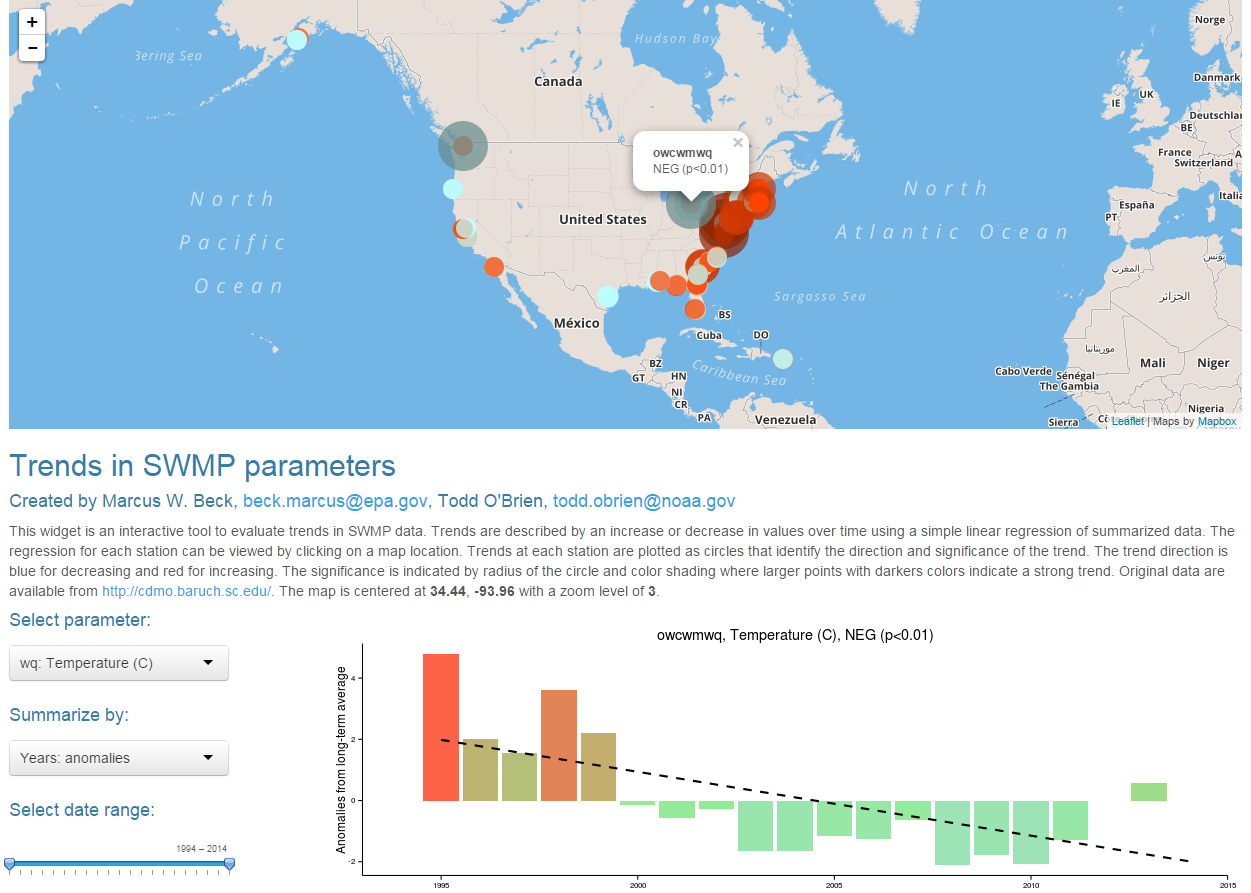
\includegraphics[width = 0.75\textwidth]{fig/swmp_comp.png}}
\end{frame}

%%%%%%
\begin{frame}{Conclusions}
Shiny has multiple benefits:\\~\\
\begin{columns}
\begin{column}{0.8\textwidth}
\begin{itemize}
\item Increased accessibility to information within and outside of the research community \\~\\
\item Available for use with minimal or no experience in web programming \\~\\
\item All open-source, no need for license and under active development \\~\\
\end{itemize}
\end{column}
\begin{column}{0.2\textwidth}
\centerline{
\includegraphics[width = \textwidth]{fig/shiny_logo.png}}
\end{column}
\end{columns}
\vspace{0.16in}
Opportunities for EPA Shiny Server?
\end{frame}

%%%%%%
\begin{frame}{Additional resources}
RStudio Shiny tutorial:\\ \url{http://shiny.rstudio.com/tutorial/} \\~\\
RStudio Shiny gallery:\\ \url{http://shiny.rstudio.com/gallery/} \\~\\
Deploy Shiny apps: \\ \url{http://www.shinyapps.io/} \\~\\
This presentation (\url{beck.marcus@epa.gov}):\\ \url{https://github.com/fawda123/shiny_pres/raw/master/shiny_pres.pdf}
\end{frame}

\end{document}
